\chapter{esfericas}

%%%%%%%%%%%%%%%%%%%%%%%%%%%%%%%%%%%%%%%%%%%%%%%%%%
\section{Introduction}
%%%%%%%%%%%%%%%%%%%%%%%%%%%%%%%%%%%%%%%%%%%%%%%%%%


The design of functional vehicles for the encapsulation, transport and release on target of therapeutic agents is one of the major challenges of bionanotechnology \addcite[ye2018review].
Despite being formulated to specifically treat certain diseases, many drugs fail to capitalize on their design properties due to  unwanted interactions with the environment surrounding the target \addcite[ibraheem2014administration].
Nanoparticles are being explored as a solution to these limitations, serving as smart carriers that can  protect drugs against harmful environmental factors.
Various nanocarriers, including liposomes, polymeric micelles, and inorganic particles have been investigated for their potential to effectively transport and release molecular cargo \addcite[chamundeeswari2019nanocarriers, lopez2012organic].
These nanocarriers can increase circulation time while conferring stealth properties to the complex, helping evade the immune or digestive systems \addcite[gaucher2010polymeric].
By increasing the circulation time, nanocarries can also help reduce the need for frequent dosing.






Nanogels, in particular, are soft nanoparticles with diameters smaller than 200\,nm that can uptake and release relatively large quantities of solvent in response to changes in the surrounding environment.
Depending on the chemical composition of the crosslinked polymer that makes the nanogel skeleton, these particles can reversibly swell or deswell as a result of changes in temperature \addcite[agnihotri2021temperature], pH \addcite[sharma2022modulating], salt concentration \addcite[saraydin2022calculations] and a variety of external stimuli \addcite[jung2020responsive,plamper2017functional, yang2022co].
These unique properties of polymer nanogels can be exploited to target drug delivery to specific microenvironments, such as the acidic surroundings of tumors \addcite[zhang2020construction] or wounded or inflamed tissue with higher temperatures \addcite[wu2010core].
Besides, moieties can be incorporated on its polymeric surface to enhance specificity of the delivery, allowing the nanogel to selectively bind receptors on the target \addcite[ahadian2020micro, mukherjee2019lipid, torchilin2007micellar, farokhzad2006targeted].
The ability of nanogels to release medication in a controlled manner to specific environments can help prevent the emergence of drug resistance \addcite[mukherjee2019lipid].







A significant and growing fraction of newly developed drugs to treat different diseases are proteins \addcite[mahmood2023recent].
The stability of these proteins is an issue, as they are easily denatured by changes in pH or temperature \addcite[frokjaer2005protein].
Polymer hydrogels and nanogels have been shown to help prevent protein denaturation and loss of activity under these conditions \addcite[macdougall2021charged, peppas2004hydrogels].
The potential to maintain the native conformation of proteins, combined with the stimuli-responsive behavior of nanogels, makes them suitable candidates to develop functional vehicles for the encapsulation, transport and targeted release of therapeutic proteins.
Additionally, the polymer network of nanogels can be tailored with different functional groups to control both the specific or non-specific  interactions with proteins, thereby increasing the efficacy of encapsulation/delivery.



Despite their many advantages, the development of nanogel-based drug delivery systems is still in its early stages, and there are still many questions that need to be addressed before this technology can be fully realized.
In particular, as they are required to function in various biological fluids, understanding how nanogels behave and interact with proteins in terms of the composition of its polymer network and that of the  protein solution is crucial for their successful application.
In this work, we use a theoretical approach to study how the chemical identity and the spatial distribution of functional groups on the polymer network modify nanogel response and its interaction with specific proteins, with a specific focus on electrostatically driven protein adsorption/desorption.
Our goal is to provide a better basic understanding of the factors that influence the performance of these systems and to identify strategies to improve their effectiveness in the context of drug delivery nanovehicles.






We consider nanogels made of copolymer networks containing both a hydrophilic, charge-neutral monomer and a pH-responsive one, and their interactions with small globular proteins, such as cytochrome c, insulin, and myoglobin, which have different isoelectric points.
ROJO
	The interaction of these proteins with polymeric systems have been studied previously \addcite[hagemann2018use,oberle2015competitive].
	These polymeric systems have also been studied using the theory and molecular simulations.\addcite[sharma2022modulating,hofzumahaus2021monte,polotsky2013collapse, walkowiak2020thermodynamic]
ROJO
In particular, the search for more effective and less invasive means of insulin administration has presently immense importance in biomedical research \addcite[lowman1999oral,wong2018microparticles,chaturvedi2013polymeric].




We study nanogels based on copolymers of vinyl alcohol (VA) and either a methacrylic acid (MAA; proton donor) or allylaimine (AH; proton acceptor).
Due to their biocompatibility these monomers are widely used for potential drug delivery applications \addcite[asadi2020common,sarwar2020smart,lowman1999oral].
With the goal of gaining a deeper understanding of the factors that affect the performance of these systems and identifying strategies for adjusting their interactions with different proteins, we derive and apply a statistical thermodynamic theory that allows for a molecular-level description of all chemical species.
This method incorporates an explicit description of network conformations that result in elasticity, ion and solvent confinement entropic effects, acid-base equilibrium chemistry as well as electrostatic interactions and steric repulsions.
Specifically, we investigate the effect of the spatial distribution of pH-sensitive units through the polymer network on the nanogel swelling and protein adsorption.















%%%%%%%%%%%%%%%%%%%%%%%%%%%%%%%%%%%%%%%%%%%%%%%%%%
\section{Method: Molecular Theory}
%%%%%%%%%%%%%%%%%%%%%%%%%%%%%%%%%%%%%%%%%%%%%%%%%%



%%%%%%%%%%%%%%%%%%%%%%%%%%%%%%%%%%%%%%%%%%%%%%%%%%
\subsection{Theoretical Framework}\label{sect:theory}
%%%%%%%%%%%%%%%%%%%%%%%%%%%%%%%%%%%%%%%%%%%%%%%%%%


 

This study presents a self-consistent molecular theory to address the effect of the spatial distribution of pH-responsive groups on the thermodynamics of  protein adsorption to polymer nanogels.
This theory is based on the developments of Szleifer and collaborators to study weak polyelectrolyte surfaces \addcite[nap2006weak,Gong2007PRL].
We have previously extended this method to investigate the adsorption of proteins to pH-responsive hydrogel films \addcite[hagemann2018use,longo2019protonation].
Here, we generalize the approach to describe the behavior of nanogels made of crosslinked pH-responsive copolymer chains in contact with a protein solution.
 


This method involves minimizing a generalized free energy that includes all relevant physical chemistry.
Additionally, it incorporates a coarse-grained molecular characterization of the various chemical species present in the system, including their shape, size, charge distribution, and protonation state.
The system under study is a single nanogel in equilibrium with an aqueous solution having externally defined bulk composition.
Namely, the pH, salt concentration and protein concentration are the independent variables.
The polymer network that gives structure to the nanogel  contains two types of segments: a pH-sensitive unit, either acidic (MAA) or basic (AH), and neutral segment (VA); 
crosslinks are described as charge neutral segments.
The semi-grand potential of this system contains the following contributions:
\begin{align}
\begin{aligned}
\Omega_{NG}=& -TS_{mix} -TS_{conf,nw} + F_{chem,nw} + F_{chem,pro}\\
& + U_{elec} + U_{ste}  - {\sum_{\gamma}{\mu_\gamma N_\gamma}}
\end{aligned}
\label{eq:semicano}
\end{align}
\noindent where $S_{mix}$ is the translational (mixing) entropy of the solution species: water molecules (H$_2$O), hydronium ions (H$_3$O$^+$), hydroxide ions (OH$^-$), salt cations, salt anions and proteins.
We consider a monovalent salt, NaCl, and assume it is completely dissociated into sodium (Na$^+$) and chloride ions (Cl$^-$).
$S_{conf,nw}$ represents the conformational entropy that results from the flexibility of the polymer network, which can assume many different conformations. 
$F_{chem,nw}$ is the chemical free energy that describes the equilibrium between the protonated and deprotonated species of functional (acid/basic) units on the polymer. 
Similarly, $F_{chem,pro}$ describes the protonation of titratable residues of the protein.
$U_{elec}$ and $U_{ste}$ account, respectively, for the electrostatic interactions and steric repulsions.
Finally, the sum over $\gamma$ expresses the chemical equilibrium between our system and the bulk solution that represent a bath for the free particles, where $\mu_\gamma$ and $N_\gamma$ are the chemical potential and number of molecules of species $\gamma$, respectively;
the subindex $\gamma$ runs over the free chemical species, including proteins.
Note that $\Omega_{NG}$ is a semi-grand potential because the nanogel  can exchange each of these free molecules with the bulk solution, while the polymer network is confined within our system.
A detailed derivation of the theory can is presented in the SI.










%%%%%%%%%%%%%%%%%%%%%%%%%%%%%%%%%%%%%%%%%%%%%%%%%%
\subsection{Molecular Model: Proteins}\label{sect:protein}
%%%%%%%%%%%%%%%%%%%%%%%%%%%%%%%%%%%%%%%%%%%%%%%%%%


We consider three different proteins:  cytochrome c, insulin and myoglobin.
To describe these molecules we use a coarse-grained model where each amino acid residue is described by a single particle centered at the position of the $\alpha$-carbon.
The sequence and position of all $\alpha$-carbons are taken from the crystallographic structure in the corresponding protein data bank entry \addcite[berman2000protein]: 2B4Z for cytochrome c \addcite[mirkin2008high], IZNI for insulin \addcite[bentley1976structure], and 3RGK for myoglobin \addcite[hubbard1990x]. 
 
 

The coarse-grained particles in this model are each assigned a volume and a pKa (if the unit is titratable) according to the amino acid that they represent; 
this is summarized in  tabla \ref{table:Coarse-grain}.
These pKa's are taken from experimental data and represent average values over a large number of proteins \addcite[grimsley2009summary].
In most occurrences of a residue, its pKa does not significantly deviate from the average value.
In  specific instances, however, some residues display a different pKa;
these special cases are described in the SI.


\begin{table}
\centering
\small
\begin{tabular}{|lcc|lcc|}
\hline
grupo & v($nm^{-3}$) & pka & grupo & v($nm^{-3}$) & pka \\
\hline
Ala & 0.067 &  & Pro & 0.090 & \\
Arg & 0.148 & $12.5 (+)$& Ser & 0.073 &\\
Asn & 0.096 &  & Thr & 0.093 & \\
Asp & 0.091 & $3.5 (-)$ & Trp & 0.163 &\\
Cys & 0.086 &  & Tyr & 0.141 & $10.3 (-)$\\
Gln & 0.114 & & Val & 0.105 &\\  
Glu & 0.109 & $4.2 (-)$ & H$_2$O & 0.033 & \\ 
Gly & 0.048 &  & OH$^-$ & 0.033 & \\
His & 0.118 & $6.6 (+)$& H$_3$O$^+$ & 0.033 &  \\ 
Ile & 0.124 &  & Na$^+$ & 0.043 & \\ %
Leu & 0.124 &  & Cl$^-$ & 0.047 & \\
Lys & 0.135 & $10.5 (+)$ & AH & 0.068 &  9.5(+)\\
Met & 0.124 & & MAA & 0.085 & $4.65(-)$\\
Phe & 0.135 &   & VA & 0.085 & \\
\hline
\end{tabular}
\caption{Volume and pKa of the coarse-grained particles (amino acid residues, small ions, solvent molecules and polymer segments)  considered in our molecular model.}
\label{table:Coarse-grain} 
\end{table}


Using this molecular model,  figura \ref{fig:protein-charge} shows the charge (number) of the three proteins in dilute solution as a function of  pH.
The isoelectric point (pI) is the pH at which the net charge of a protein is zero.
From the graph, we obtain the values  9.65 (9.6 \addcite[hristova2019isoelectric]), 5.5 (5.3 \addcite[guckeisen2019isoelectric]), 7.15 (7.2 \addcite[batys2020myoglobin]) for the pI of cytochrome c, insulin, and myoglobin respectively;
the values in parentheses are the pI of the proteins reported experimentally. 


 \begin{figure}[!htb]
     \centering
     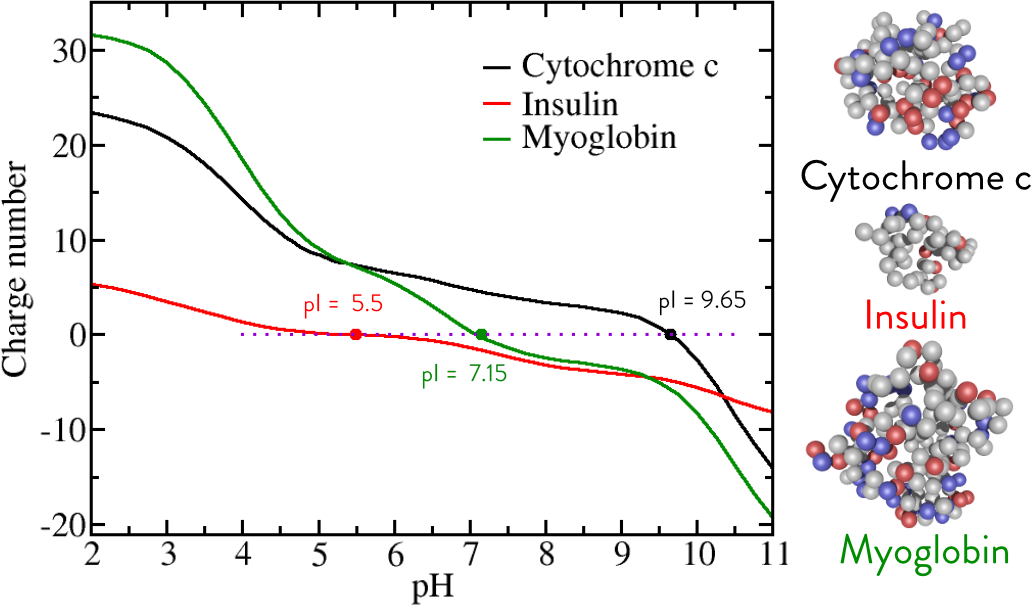
\includegraphics[width=0.65\textwidth]{Figures/graphs-gel2/protein-model.png}
     \caption{Left: Charge number of the proteins in a dilute solution as a function of  pH (solid-line curves);
     filled circles mark  the isoelectric point,
     where the net charge of the protein is zero.
     The coarse-grained representation of the proteins is illustrated on the right, where amino acid residues are represented by a single sphere (red: acidic; blue: basic; gray: charge-neutral residues).}
     \label{fig:protein-charge}
 \end{figure}






 





%%%%%%%%%%%%%%%%%%%%%%%%%%%%%%%%%%%%%%%%%%%%%%%%%%
\subsection{Molecular model: Nanogel Network}
%%%%%%%%%%%%%%%%%%%%%%%%%%%%%%%%%%%%%%%%%%%%%%%%%%

Besides the protein model presented in sec.  \ref{sect:protein},   we need to specify a molecular model to describe the polymer network that makes the nanogel backbone.
Such model must provide  a set of molecular configurations of the polymer network that is representative of the whole conformational space.
A particular network conformation is given by the spacial position of all its segments.


The nanogel network is composed of 25 segment-long  crosslinked polymer chains. 
In total this network contains 10054 segments.
Each segment is a coarse-grained   representation of either a crosslink, a charge neutral unit (VA) or an acid/basic monomer (MAA/AH). 
tabla \ref{table:Coarse-grain} includes the volume and pKa (if the unit is titratable) used to describe these coarse-grained units.

The polymer network has diamond-like topology, where  crosslinks are placed at the original position of carbon atoms and connected to four polymer chains.
To build this network, we first construct a three-dimensional structure where all the polymer chains are elongated, to then only keep the segments contained within a sphere of radius $R_{cut}$ placed at the center of mass of the structure; $R_{cut}$ is selected such that the network will have 10000 segments approximately.
Originally, all polymer chains connect two crosslinks, but as a result of this procedure some will be left dangling on the network surface,  connected to a single crosslink.
Most of these superficial \emph{dangling} chains are shorter than 25 segments.
Altogether these chains contain 22\% of the total number of segments.
To generate the different molecular conformations of the polymer network, we have performed Molecular Dynamics simulations using GROMACS 5.1.2 \addcite[indahl2001gromacs] (details are given in the SI).

 \begin{figure}[!htb]
     \centering
     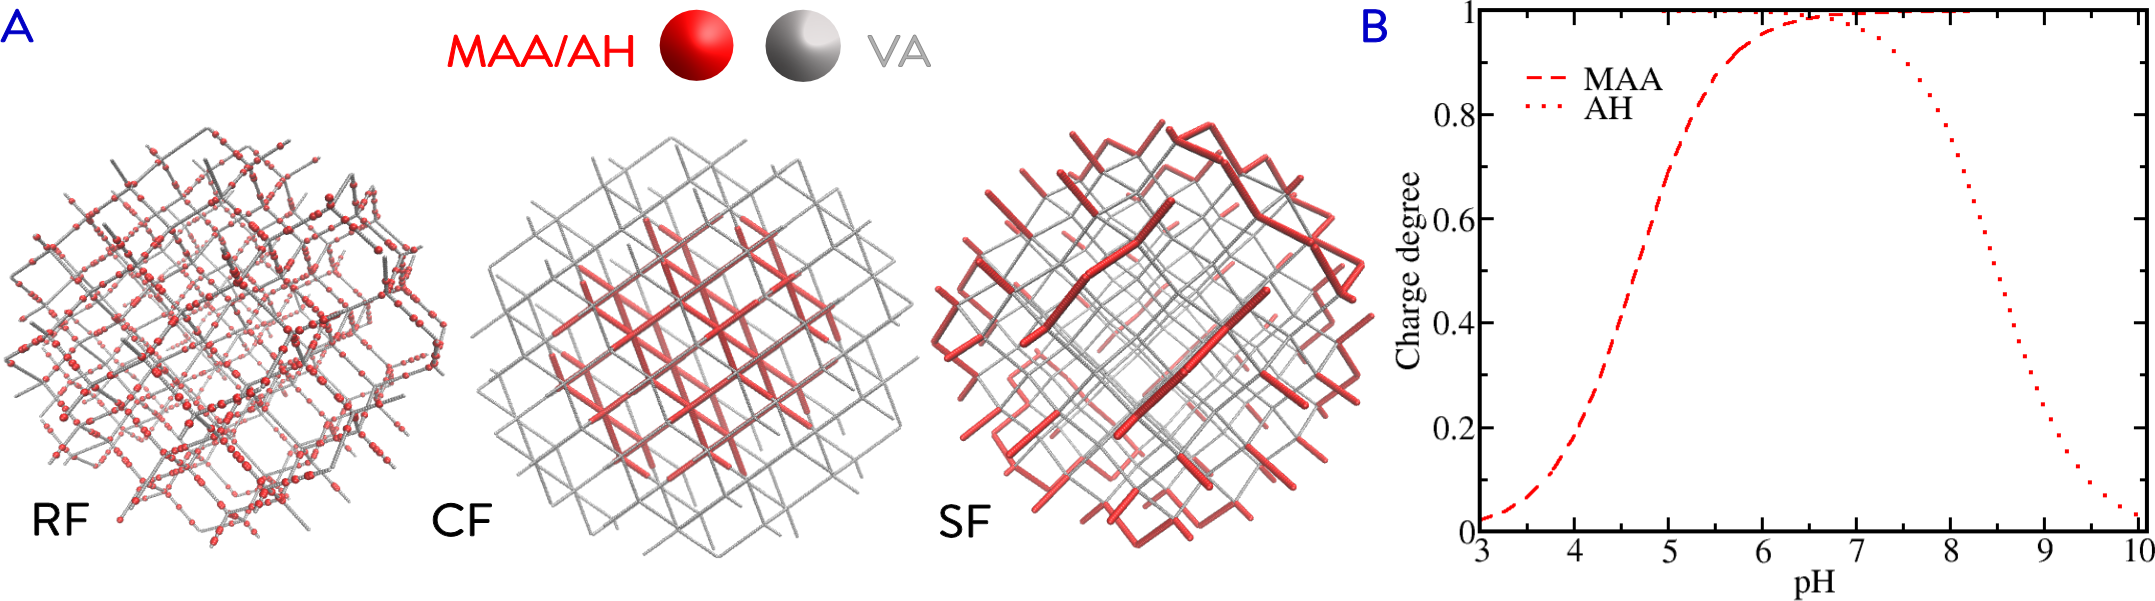
\includegraphics[width=0.99\textwidth]{Figures/graphs-gel2/paper2.png}
     \caption{A: The nanogel network consists of crosslinked copolymer chains of a charge-neutral segment (VA: vinyl alcohol) and a functional unit (either MAA: methacrylic acid or AH: allylamine).
    This scheme illustrates the three different comonomer distributions considered;  from left to right: RF: a random distribution of functional groups throughout the network; CF: the functional units occupy the center/core of the network; SF: only the free-end dangling chains on the network surface are functionalized with pH-responsive units.
B: Plot of the ideal pH-dependent degree of charge of the isolated functional unit in dilute solution.}
     \label{fig:gel-topologies}
 \end{figure}














We consider different pH-responsive nanogels, containing either acid (MAA) or basic (AH) groups, and evaluate three different topologies for the spatial distribution of these functional  segments, which are schematized in figura \ref{fig:gel-topologies}: 
(i) a \emph{randomly functionalized} (RF) structure where the pH-responsive segments are spread throughout the network  at random,
(ii) a \emph{core functionalized} (CF) structure, where the  pH-sensitive units occupy the center of the network, and 
(iii) a \emph{surface functionalized} (SF) structure in which only the dangling chains on the network surface  are ionizable. 

 
 
  







%%%%%%%%%%%%%%%%%%%%%%%%%%%%%%%%%%%%%%%%%%%%%%%%%%
\section{Results and discussion}
%%%%%%%%%%%%%%%%%%%%%%%%%%%%%%%%%%%%%%%%%%%%%%%%%%






%%%%%%%%%%%%%%%%%%%%%%%%%%%%%%%%%%%%%%%%%%%%%%%%%%
\subsection{Nanogel response}
%%%%%%%%%%%%%%%%%%%%%%%%%%%%%%%%%%%%%%%%%%%%%%%%%%
Primero, examinaremos el comportamiento de los nanogeles en funci\'on del pH cuando no hay prote\'inas presentes.
Para cuantificar el tama\~no de un nanogel, usamos el radio promedio conjunto de la partí\'icula, $R$, que se puede calcular usando:
\begin{align}
    R= \frac{4}{3}\frac{\int_0^\infty{dr\,G(r)\,r \left<\phi(r)\right>}}{\int_0^\infty{dr\,G(r)\left<\phi(r)\right>}}
\end{align}
donde $r$ es la distancia desde el centro de masa de la red polim\'erica (nuestra teor\'ia asume simetr\'ia radial);
$\left<\phi(r)\right>$ es la fracci\'on de volumen local del pol\'imero que incluye todos los tipos de segmentos, ionizables y de carga neutra;
los corchetes angulares indican el promedio del conjunto sobre las diferentes conformaciones de la red;
$G(r)=4\pi r^2$ es el \'area superficial de la esfera de radio $r$.

\begin{figure}[!htb]
     \centering
     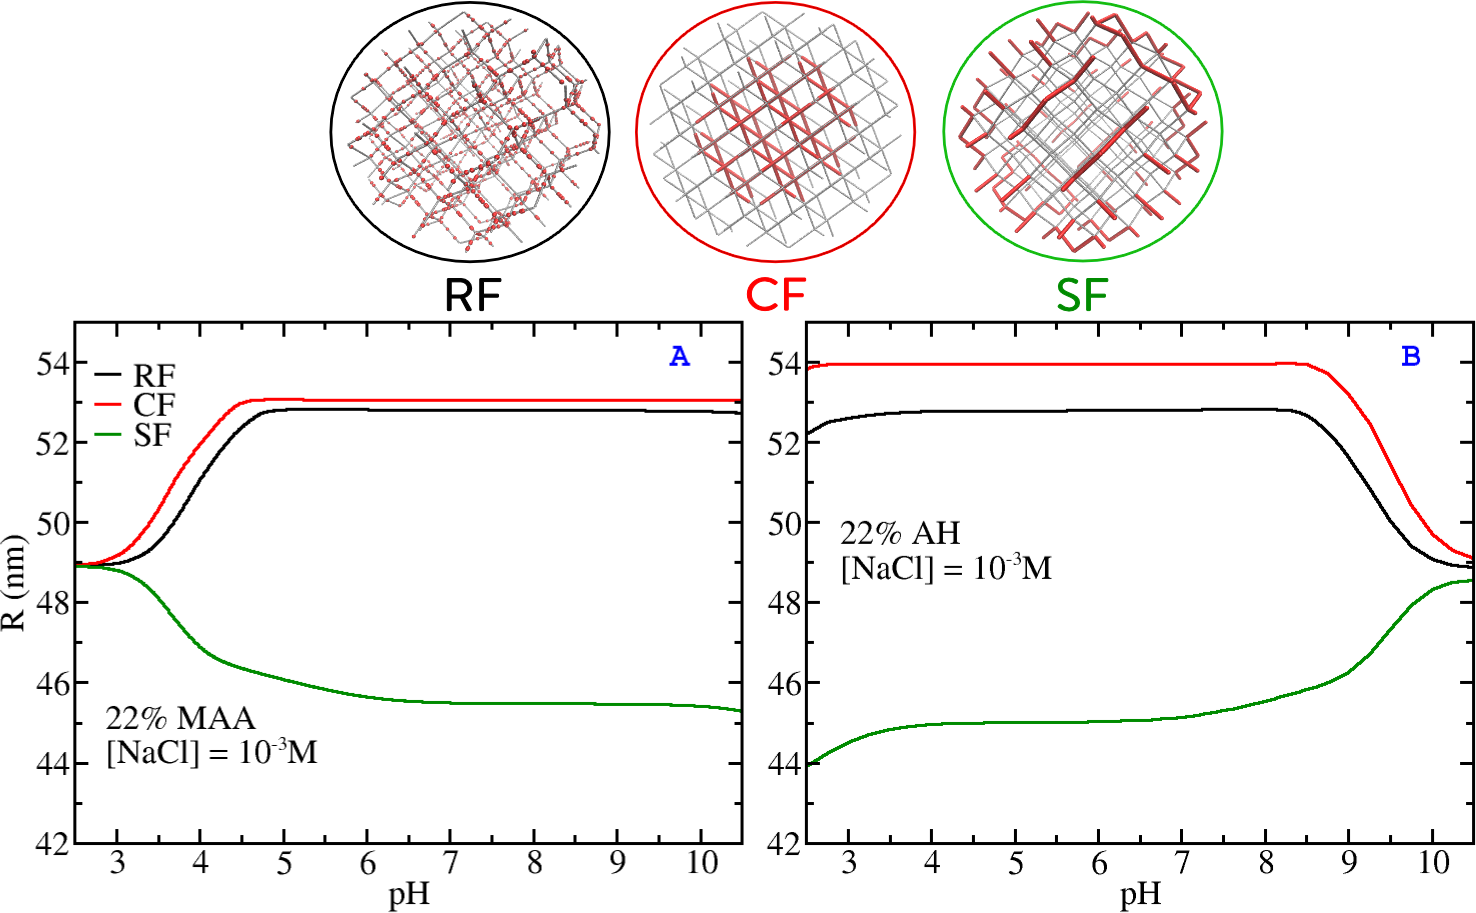
\includegraphics[width=0.9\textwidth]{Figures/graphs-gel2/rr.png}
     \caption{Conjunto de radio promedio, R, en funci\'on del pH para nanogeles de copo\'imero MAA-VA (panel A) y AH-VA (panel B).
     	Se consideran tres estructuras diferentes en cada caso donde las unidades funcionales (MAA/AH) se distribuyen aleatoriamente a lo largo de la red polim\'erica (RF), ocupan el centro de la red (CF), o modifican las cadenas colgantes dentro del pol\'imero. interfaz de soluci\'on (SF).
     	En todos los casos, el $22\%$ de los segmentos de estas redes son sensibles al pH; La concentraci\'on de NaCl es $10^{-3}M$.}
     \label{fig:gel-charge-MAA-AH}
\end{figure}

La Figura \ref{fig:gel-charge-MAA-AH} muestra $R$ en funci\'on del pH para las tres diferentes estructuras consideradas: RF, CF y SF.
El panel A describe un nanogel basado en MAA, mientras que el panel B describe un nanogel basado en AH.
En ambos casos, la concentraci\'on de sal es de 1\,mM, y la fracci\'on de mon\'omero funcional (MAA o AH) es de $22\%$.
Los nanogeles basados en MAA funcionalizados al azar y en el n\'ucleo se hinchan al aumentar el pH (panel A).
Esto se debe a que los segmentos MAA se desprotonan y se cargan el\'ectricamente a medida que aumenta el pH (ver figura \ref{fig:gel-topologies}B), lo que da como resultado repulsiones electrost\'aticas dentro de la red.
La distancia entre las unidades MAA cargadas debe aumentar para reducir estas interacciones repulsivas, y la red aumenta para colocar estos segmentos m\'as separados.
Para disminuir la repulsi\'on entre unidades MAA cargadas, su distancia espacial debe aumentar, lo que resulta en una expansión neta de la red.




La red MAA funcionalizada en superficie, por otro lado, muestra un comportamiento de expansi\'on completamente diferente en figura \ref{fig:gel-charge-MAA-AH}A.
Este nanogel se deshincha a medida que las unidades titulables se cargan al aumentar el pH.
Para explicar este comportamiento contrario a lo que se espera, observamos la distribuci\'on local de pol\'imeros dentro de estas estructuras en diferentes condiciones.
Para ello, utilizamos la distribuci\'on radial de los mon\'omeros funcionales.
Para los nanogeles MAA, dicha cantidad se define como:

%
\begin{align}
    \lambda_{MAA}(r)= 4\pi r^2\left<\phi_{MAA}(r)\right>
\end{align}
%
\noindent en donde $\left<\phi_{MAA}(r)\right>$ da la fracci\'on de volumen local de los segmentos de \'acido metacr\'ilico.
Hay que tener en cuenta que $\lambda_{MAA}(r) dr$ da el n\'umero de segmentos MAA en la capa esf\'erica entre $r$ y $r+dr$ medidos desde el centro del nanogel.
Adem\'as, la integral $\int_0^\infty \lambda_{MAA}(r) dr$ da el n\'umero total de mon\'omeros MAA en la red.


\begin{figure}[!htb]
     \centering
     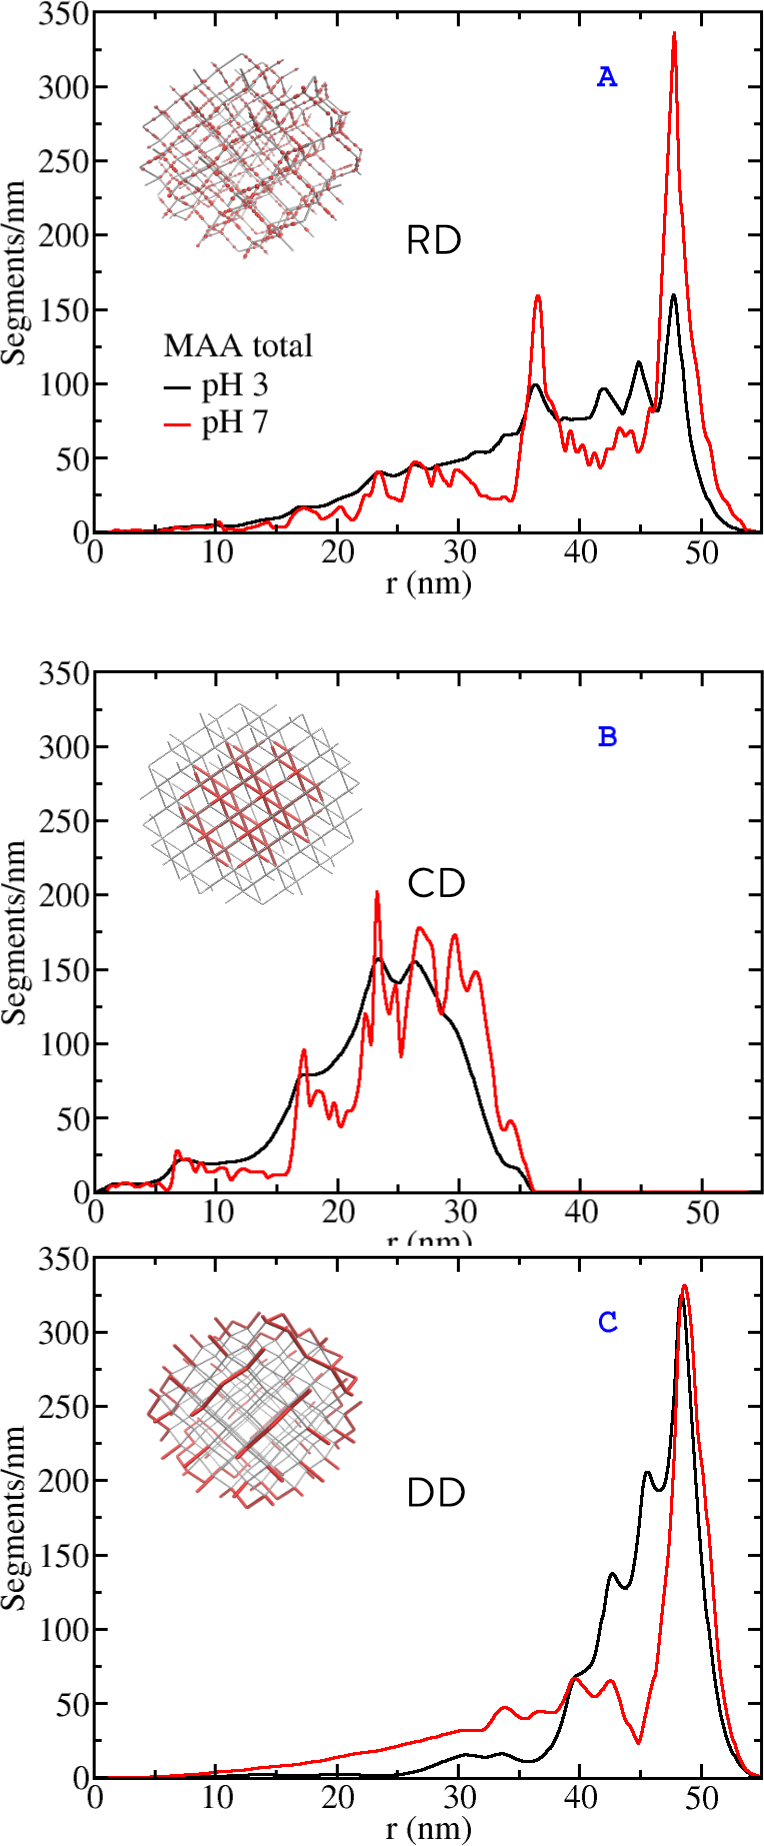
\includegraphics[width=0.45\textwidth]{Figures/graphs-gel2/dist-MAA.png}
     \caption{Distribuci\'on radial de segmentos MAA, $\lambda_{MAA}(r)$, a pH 3 y 7, y $10^{-3}M$ NaCl; cada panel corresponde a un nanogel de  MAA-VA diferente que tienen una funcionalizaci\'on de red particular y 22\% MAA.
     	Estos grupos funcionales est\'an completamente protonados (sin carga) a pH 3 y completamente disociados (cargados) a pH 7.}
     \label{fig:MAA-vs-r-distribution}
 \end{figure}
 %\FloatBarrier


La figura \ref{fig:MAA-vs-r-distribution} muestra la distribuci\'on radial de los segmentos MAA para las diferentes redes consideradas.
En cada caso incluimos resultados para una solución de pH 3, donde los segmentos MAA tienen carga neutra, y pH 7 donde est\'an completamente cargados;
el pKa intr\'inseco de MAA es 4,65.
Para una funcionalizaci\'on aleatoria (panel A), la distribuci\'on de los segmentos MAA se desplaza hacia la interfaz de soluci\'on de nanogel a medida que la red se carga el\'ectricamente cuando aumenta el pH.
Como se mencion\'o anteriormente, este desplazamiento se produce para reducir las repulsiones electrost\'aticas entre los segmentos MAA cargados.
%Tenga en cuenta que el volumen del caparazón que contiene estos segmentos aumenta con $r$.
Como resultado, toda la distribuci\'on del pol\'imero tambi\'en se extiende %(ver \cref*{fig:allseg_si}\hl{A y B en el SI})
, incluidas las unidades VA de carga neutra.
El mismo comportamiento tiene lugar para una funcionalizaci\'on central (panel B),
aunque por dise\~no, los segmentos MAA en esta red, ya sea que est\'en cargados o no, es m\'as probable que ocurran a distancias m\'as cortas del centro del nanogel en comparaci\'on con las otras estructuras.
El desplazamiento del segmento a $r$ m\'as altos observado en los paneles figura \ref{fig:MAA-vs-r-distribution}A y B explica el aumento del tama\~no promedio del nanogel con pH visto en la figura \ref{fig:gel- charge-MAA-AH}A para las estructuras RF y CF.


Por otro lado,
La Figura \ref{fig:MAA-vs-r-distribution}C muestra que la distribuci\'on MAA del nanogel con superficie funcionalizada se desplaza hacia adentro cuando la red se carga con pH.
Para reducir las repulsiones dentro de la red, las cadenas lindantes de PMAA, que se asientan en la superficie del nanogel a un pH bajo, tambi\'en intentan ocupar el volumen dentro de la red cuando están cargadas.
Este cambio hacia adentro de la distribuci\'on de segmentos de pol\'imero %(\hl{ver también} \cref*{fig:allseg_si}C)
explica el comportamiento de deshinchamiento del nanogel SF MAA con el aumento del pH que se observa en la figura \ref{fig:gel-charge-MAA-AH}A.
N\'otese, sin embargo, que a pesar de este desplazamiento parcial hacia el interior de la red, la posici\'on m\'as probable de los segmentos MAA es siempre la interfaz pol\'imero-soluci\'on para soluciones de pH alto y bajo.



El comportamiento de los nanogeles basados en AH es an\'alogo al de las redes basadas en MAA, pero en respuesta al cambio de pH en la direcci\'on opuesta.
Los grupos AH se protonan y se cargan positivamente con la disminuci\'on del pH (ver figura \ref{fig:gel-topologies}B).
Para nanogeles AH funcionalizados aleatoriamente y con n\'ucleo, este aumento en la carga el\'ectrica con la disminución del pH provoca un desplazamiento hacia afuera de la distribuci\'on del segmento % (ver \cref*{fig:AHseg_si}A y B)
, lo que explica la hinchaz\'on de la figura \ref{fig:gel-charge-MAA-AH}B;
mientras tanto, para la estructura SF, el deshinchamiento con la disminuci\'on del pH que se ve en la figura \ref{fig:gel-charge-MAA-AH}B es consistente con un desplazamiento hacia adentro del pol\'imero %(ver \cref*{fig:AHseg_si}C) .





%%%%%%%%%%%%%%%%%%%%%%%%%%%%%%%%%%%%%%%%%%%%%%%%%%
\subsection{Protein adsorption to MAA-based nanogels}\label{sec:MAA-NGs}
%%%%%%%%%%%%%%%%%%%%%%%%%%%%%%%%%%%%%%%%%%%%%%%%%%



%%%%%%%%%%%%%%%%%%%%%%%%%%%
%%%%% Define Gamma and N(r)
%%%%%%%%%%%%%%%%%%%%%%%%%%%

En la secci\'on anterior eval\'ua el impacto de la funcionalizaci\'on de la red y la composici\'on qu\'imica en la respuesta del nanogel a las variaciones de pH en ausencia de prote\'inas.
La reorganizaci\'on de los segmentos de pol\'imero como resultado de los cambios de pH depende de una elecci\'on de dise\~no: la distribuci\'on de unidades funcionales dentro de la red.
Ahora examinaremos el impacto de esta reorganizaci\'on de pol\'imeros en el nivel de adsorci'on de prote\'inas en diferentes nanogeles y la distribuci\'on espacial de las prote\'inas adsorbidas.
Esta secci\'on analiza la adsorció\'on del citocoma c y la mioglobina en diferentes estructuras de nanogel basadas en MAA.
Los resultados de la insulina se omiten en esta secci\'on porque, debido a su bajo punto isoel\'ectrico, esta prote\'na no se adsorbe en nanogeles basados en MAA. % (see fig. \cref*{fig:adsoprtion-vs-pH-insulinMAA_si} in the SI).

Considere un nanogel polim\'erico centrado en $r=0$ en contacto con una soluci\'on acuosa de prote\'ina.
El n\'umero de prote\'inas adsorbidas dentro de la capa esf\'erica entre $r$ y $r+dr$ viene dado por la cantidad en exceso

\begin{align}
     \langle N(r)\rangle dr = 4\pi r^2 \left(\langle\rho(r)\rangle - \rho_{bulk}\right) dr
\end{align}
%
en donde $\left<\rho(r)\right>$ y $\rho_{bulk}=\lim\limits_{r\to \infty } \langle\rho(r)\rangle$ son respectivamente la densidad (en n\'umero) local y en el bulk de la prote\'ina.
La integraci\'on de $\langle N(r)\rangle$ produce la \emph{adsorci\'on en exceso} (en adelante, simplemente la adsorci\'on) que cuantifica el n\'umero de prote\'inas incorporadas a la red de pol\'imeros,


%
\begin{align}
    \Gamma =  \int_0^\infty{  \langle N(r)\rangle dr}
\end{align}
%

%%%%%%%%%%%%%%%%%%%%%%%%%%%
%%%%% Adsorption to MAA NGs
%%%%%%%%%%%%%%%%%%%%%%%%%%%


\begin{figure}[!htb]
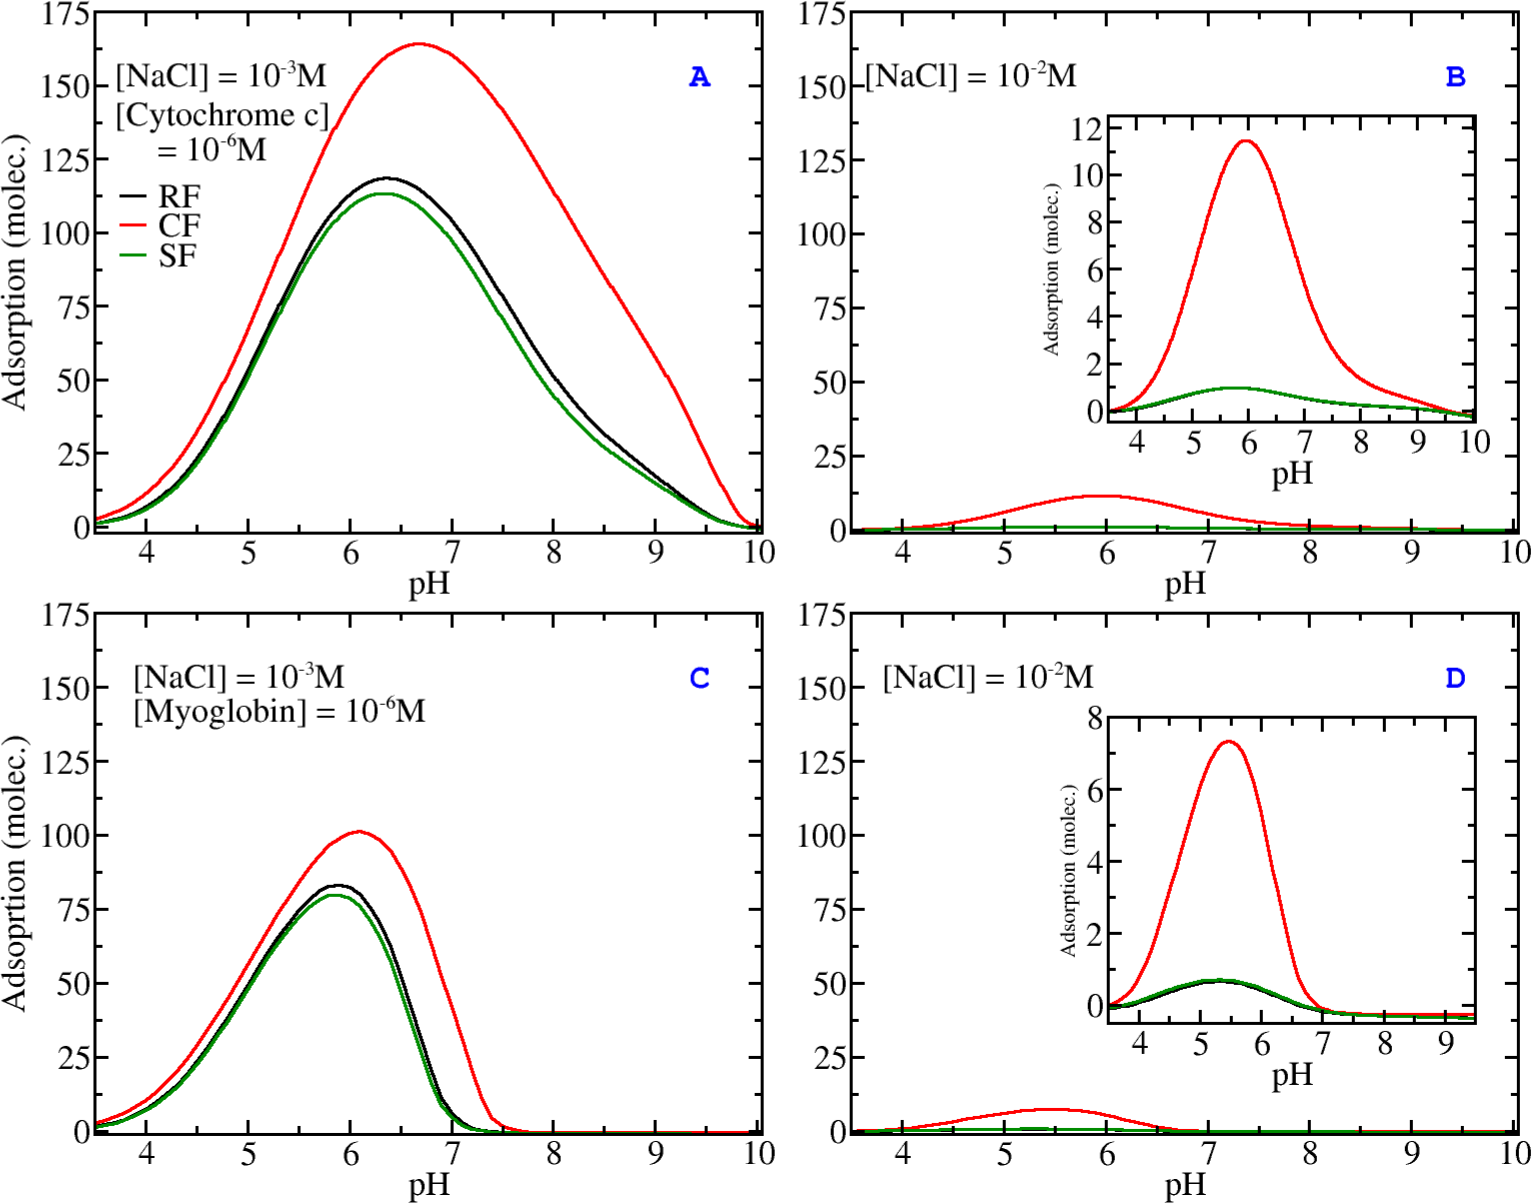
\includegraphics[width=0.9\textwidth]{Figures/graphs-gel2/abcd.png}
\caption{Gr\'aficos del exceso de adsorci\'on $\Gamma$ de citocromo c (paneles A y B) y mioglobina (paneles C y D) a nanogeles MAA-VA en funci\'on del pH.
	La concentraci\'on de sal es $10^{-3}M$ en los paneles del lado izquierdo (A y C) y $10^{-2}M$ en los paneles del lado derecho
	(B y D); Se muestra una ampliaci'on de la adsorci\'on.
	Estos nanogeles tienen 22\% MAA; la concentraci\'on de prote\'ina es $10^{-6}M$.}
\label{fig:adsorption-vs-pH-cyto-myo}
\end{figure}



 
 La Figura \ref{fig:adsorption-vs-pH-cyto-myo} muestra la adsorci\'on de soluciones de prote\'ina \'unica de citocromo c (paneles superiores, A y B) y mioglobina (paneles inferiores, C y D) a nanogeles MAA-VA que tienen diferentes funcionalizaciones de red;
 El pH es la variable independiente de estos c\'alculos, pero tambi\'en evaluamos el efecto de la concentraci\'on de NaCl comparando diferentes paneles en la misma l\'inea.
 Los nanogeles de Figura \ref{fig:adsorption-vs-pH-cyto-myo} contienen $22\%$ MAA, lo que significa que todos los segmentos en las cadenas superficiales de la red SF son MAA.
 Primero, discutiremos las caracter\'isticas de la figura \ref{fig:adsorption-vs-pH-cyto-myo} comunes a todos los paneles para luego concentrarnos en el efecto de la funcionalizaci\'on de la red.
 
 
 
 La adsorci\'on de prote\'inas es una funci\'on no monot\'onica del pH con un m\'aximo en la regi\'on entre pH 5-7, que depende de la concentraci\'on de sal y la prote\'ina espec\'ifica.
 Esta respuesta del pH puede explicarse en t\'erminos de las interacciones electrost\'aticas y el comportamiento de protonaci\'on tanto de los segmentos MAA como de las prote\'inas.
 Las unidades \'acidas del pol\'imero se disocian y la red se carga negativamente cuando el pH aumenta por encima de su pKa intr\'inseco (4,65 para MAA).
 Por encima de este pH, pero por debajo de su punto isoel\'ectrico, la prote\'ina tiene carga positiva.
 En estas condiciones, las atractivas interacciones prote\'ina-red impulsan la adsorci\'on.
 Sin embargo, en ambos lados de la escala de pH, estas interacciones son insignificantes (pH bajo) porque el MAA est\'a protonado y tiene carga neutra o repulsivo (pH alto) porque las prote\'inas tienen carga negativa.
 Cualquiera de las dos situaciones conduce a la ausencia de adsorci\'on de prote\'inas ($\Gamma\approx 0$) o desorci\'on ($\Gamma< 0$).
 
 
 
 En general, las adsorciones de citocromo c y mioglobina son cualitativamente similares.
 Hay dos diferencias principales: (i) la magnitud de la adsorci\'on (el citocromo c se adsorbe significativamente m\'as) y (ii) el citocromo c se adsorbe en un rango de pH m\'as amplio, lo que se debe a su punto isoel\'ectrico m\'as alto (9,65 en comparaci\'on con 7,15). para la mioglobina).
 Esto tambi\'en implica que, cuando las dem\'as condiciones son las mismas, el nivel m\'aximo de adsorci\'on de citocromo c tiene lugar a un pH ligeramente superior.
 
 En relaci\'on con las otras configuraciones, la figura \ref{fig:adsorption-vs-pH-cyto-myo} muestra que la distribuci\'on central de los segmentos MAA conduce a una adsorci\'on significativamente mayor en la mayor\'ia de las condiciones.
 Mostramos que este comportamiento ocurre porque tal distribuci\'on de segmentos MAA permite una incorporaci\'on m\'as efectiva de la prote\'ina adsorbida con carga el\'ectrica opuesta.
 Por otro lado, el comportamiento de adsorci\'on de las redes funcionalizadas aleatoriamente y de superficie es sorprendentemente similar dentro del pH y las concentraciones de sal estudiadas, y tambi\'en para las diferentes prote\'inas.
 La distribuci\'on de unidades funcionales entre estructuras RF y SF difiere mucho a pH bajo.
 Sin embargo, tras la reorganizaci\'on del polí\'imero a un pH m\'as alto a medida que se cargan las unidades MAA, estas distribuciones se vuelven relativamente similares entre s\'i (compare los paneles A y C de la Figura \ref{fig:MAA-vs-r-distribution}), lo que explica la adsorci\'on de prote\'inas comparable observado en nanogeles RF y SF.




%%%%%%%%%%%%%%%%%%%%%%%%%%
%%%%% Protein localization
%%%%%%%%%%%%%%%%%%%%%%%%%%

\begin{figure}[!htb]
     \centering
     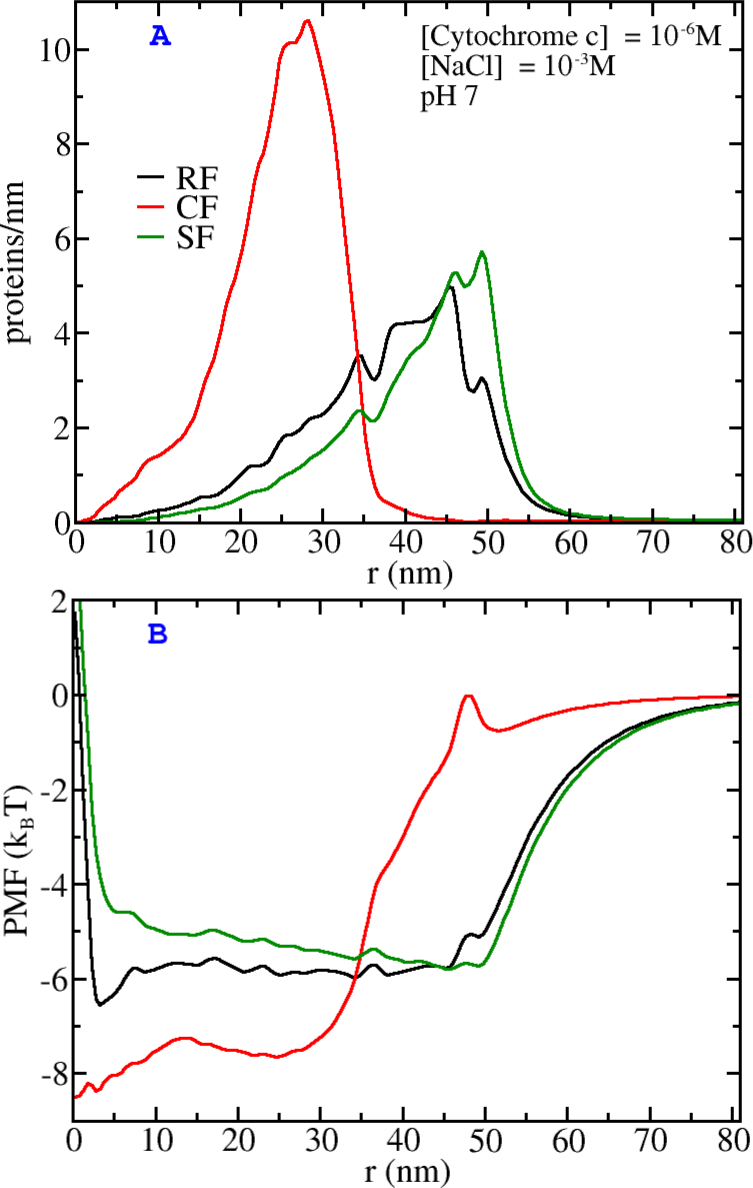
\includegraphics[width=0.45\textwidth]{Figures/graphs-gel2/cyto-adsr-pmf.png}
     \caption{Panel A: Plot of the radial distribution  of cytochrome c molecules, $\langle N(r)\rangle$, as a function of position for MAA-VA nanogels having different functionalizations.
     These networks have 22\% MAA, pH is 7, protein concentration is $10^{-6}M$, and NaCl concentration is $10^{-3}M$.
     Panel B shows the potential of mean force, ${PMF}(r)$, acting on cytochrome c for the same conditions as panel A.}
     \label{fig:adsorption-vs-r-cyto}
 \end{figure}

To explain the better performance of the core-functionalized MAA nanogels in incorporating proteins, 
Figura \ref{fig:adsorption-vs-r-cyto}A shows the radial distribution of cytochrome c molecules as a function of the distance $r$ to the nanogel center of mass.
The solution has pH 7 and 1\,mM NaCl, roughly corresponding to the conditions of maximum  adsorption of this protein in Figura \ref{fig:adsorption-vs-pH-cyto-myo}A.
There is a clear correlation between the  distribution of functional groups throughout the polymer network and the location of adsorbed cytochrome c.

When the center of the network is functionalized, the highest probability of finding the proteins occurs deep inside the nanogel between 20-30\,nm.
In Figura \ref{fig:adsorption-vs-r-cyto}A the maximum number of adsorbed proteins occurs at $r=28$\,nm for $1$\,mM NaCl, and at $r=25$\,nm for 10\,mM NaCl% (\hl{see} \cref*{fig:cyto-vs-r-1d-2_si}).
Congruently, the distribution profile of charged MAA displays a shallow maximum in this spatial region (see figura \ref{fig:MAA-vs-r-distribution}B, red curve).
Namely, adsorbed proteins sit where they can be surrounded by oppositely charged network segments.
Interestingly, the same phenomenon takes place in the adsorption to RF and SF nanogels.
The distributions of charged MAA display a sharp maximum near the nanogel surface, between 45-50\,nm (see red curves in  figura \ref{fig:MAA-vs-r-distribution}, panels A and C).
Fig 6A shows that cytochrome c is most likely to adsorb next to these  regions of high MAA (charge) density.



When comparing the distributions of cytochrome c inside RF and SF nanogels in figura \ref{fig:adsorption-vs-r-cyto}A, we observe that the profiles are relatively similar to each other.
As expected, if only the surface is functionalized, the protein profile shifts towards the polymer-solution interface.
To further quantify the interaction with the nanogels, we use the potential of mean force acting on a protein at a distance $r$ from the center of the polymer network, defined as:
\begin{align}
   {PMF} (r) = -k_B T \ln \frac{\langle \rho(r)\rangle}{\rho_{bulk}}
\end{align}
where $\lim\limits_{r\to \infty}{PMF}(r)=0$, which means that the nanogel-protein interaction vanishes when they are sufficiently far apart.





Figura \ref{fig:adsorption-vs-r-cyto}B shows ${PMF}(r)$ acting on cytochrome c at the same conditions of panel A, and for the three different nanogel functionalizations.
Deep inside the nanogel, protein interaction with the CF structure is the strongest: $-8k_B T$ approximately in the spatial range from $r=0$ to 30\,nm.
This interaction is relatively short-ranged because it decreases significantly above $r approx 40$\,nm.
On the other hand,  cytochrome c interactions with RF and SF nanogels extend longer, up to $55-60$\,nm.
Inside the nanogel, these interactions are weaker than that with the CF structure.
The adsorption free energy is $\sim -6 k_BT$ and it remains roughly constant inside the RF nanogel.
For the surface-functionalized nanogel, on the other hand, the minimum of ${PMF}(r)$ is also $\sim -6 k_BT$, occuring next to the polymer-solution interface ($r\approx 50$\,nm).
As opposed to the RF structure, this interaction is not constant inside the nanogel, but it increases monotonously as $r$ decreases and the protein gets further away from the functionalized superficial dangling chains.












%%%%%%%%%%
%%%% change in salt

\begin{figure}
     \centering
     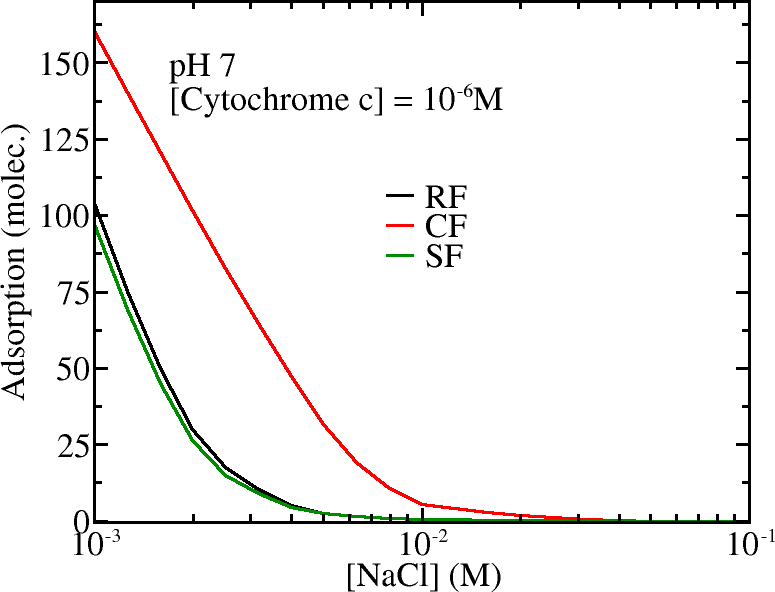
\includegraphics[width=0.45\textwidth]{Figures/graphs-gel2/gamma-salts-cyto.png}
     \caption{Plot of the excess adsorption $\Gamma$ of cytochrome c as a function of salt concentration at pH 7 for MAA-VA nanogels with different network functionalizations having 22\% MAA; protein concentration is $10^{-6}M$.}
     \label{fig:Adsorption-vs-Salt-cyto}
 \end{figure}
 

A feature of protein adsorption that we have not fully discussed yet is the effect of salt concentration.
For both cytochrome c and myoglobin, figura \ref{fig:adsorption-vs-pH-cyto-myo} shows that the incorporation of proteins inside the different nanogels is significantly enhanced by decreasing the solution salt concentration.
In order further characterize this behavior in  figura \ref{fig:Adsorption-vs-Salt-cyto} presents cytochrome c adsorption as a function of NaCl concentration at pH 7. 
This graph shows that all network functionalizations display a qualitatively similar behavior, with a dramatic decrease in adsorption between 1 and 10\,mM NaCl.
At 100\,mM all nanogels show negligible or negative adsorption.

When the solution salt concentration is high, both Na$^+$ and Cl$^-$ ions are found in high concentrations inside the nanogel.
These ions screen the electrostatic attractions between the positive charges of the protein and the negative charges on the polymer, which are the driving force for protein adsorption.
Effectively, these attractions become short range and are not strong enough to result in significant if any protein adsorption.
If the concentration of NaCl is lower, on the other hand, these electrostatic interactions are less screened and effectively longer ranged, which allows for protein adsorption.
Thus, decreasing the salt concentration enhances adsorption.
ROJO 
{Such behavior has been observed in experiments, which show that there is an increase in protein adsorption at low salt concentration \addcite[becker2012proteins, henzler2010adsorption,xu2018interaction].
Adsorption to planar and spherical polyelectrolyte brushes is significantly favored at lower salt concentrations, as demonstrated using isothermal titration calorimetry. ROJO




In considering carriers for protein delivery applications our results suggest that the best conditions for encapsulation correspond to low salt.
The adsorption profiles of figura \ref{fig:Adsorption-vs-Salt-cyto} are qualitatively similar for the three functionalizations,
but the number of proteins inside the nanogel is always significantly larger for the CF structure.
This feature may be critical in designing delivery vehicles for a target having intermediate salt concentrations.
The CF incorporates more proteins at the same conditions, but it may not be able to release them if the target has intermediate salt concentration.
For these conditions the random functionalization will be able to release all its cargo.















%%%%%%%%%%%%%%%%%%%%%%%%%%%%%%%%%%%%%%%%%%%%%%%%%%
\subsection{Insulin adsorption AH-based nanogels} 
%%%%%%%%%%%%%%%%%%%%%%%%%%%%%%%%%%%%%%%%%%%%%%%%%%




Insulin does not adsorb to the MAA nanogels of sec.  \ref{sec:MAA-NGs} %(see \cref*{fig:adsoprtion-vs-pH-insulinMAA_si} in SI).
This is because the isoelectric point of insulin and the pKa of MAA are close to each other, meaning that for solutions where the protein is positively charged, the nanogel is charge neutral, and if the nanogel is negatively charged so is the protein.
In this context, we decided to investigate insulin adsorption to an allylamine nanogel, which is positively charged below its pKa of 9.5, overlapping with the range where insulin is negatively charged.
Other than the functional monomers, the structure of these AH-VA copolymer networks is the same as that of the MAA-VA nanogels previously described.



\begin{figure}[!htb]
    \centering
    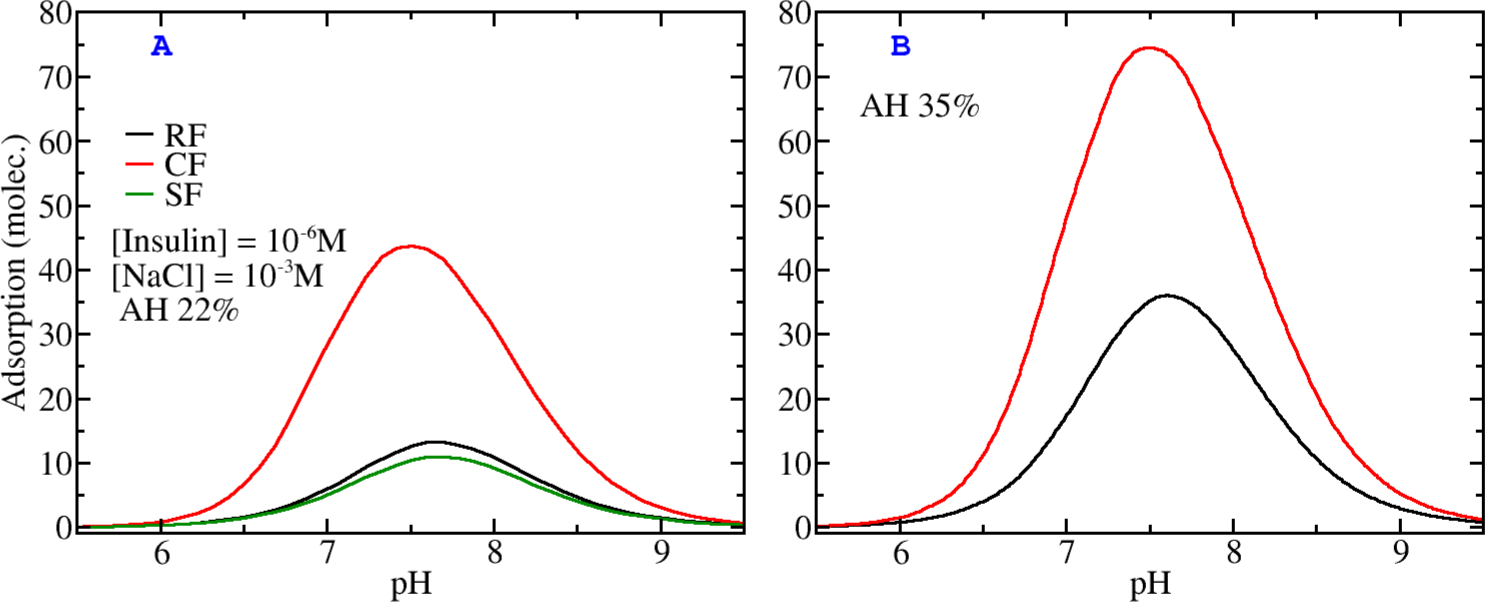
\includegraphics[width=0.9\textwidth]{Figures/graphs-gel2/insu-PAH.png}
    \caption{Plots of adsorbed insulin molecules, $\Gamma$, as a function of pH for  AH-VA nanogels having different functionalizations.
    The AH content is 22\% for the polymer networks of panel A and 35\% for those of panel B (this latter degree of functionalization cannot be achieved for the SF nanogel).
    Other conditions are $10^{-3}$\,M NaCl, and [Insulin] = $10^{-6}$\,M.}
    \label{fig:adsorption-vs-pH-insulin}
\end{figure}






Figura \ref{fig:adsorption-vs-pH-insulin}A shows the adsorption of insulin to AH-based nanogels having different spatial functionalizations.
Again we have considered networks with 22\% of pH-sensitive monomers so that we can include results for the SF nanogel, whose dangling chains are AH homo-polymers.
The main features of this plot are qualitatively similar to those of cytochrome c and myoglobin adsorption to the MAA nanogels (see Figura \ref{fig:adsorption-vs-pH-cyto-myo}).
Namely, insulin displays a  nonmonotonic adsorption as a function of the solution pH.
Moreover, we see that the core distribution of AH segments captures more insuline than either the random or the surface functionalizations.
The RF and SF nanogels display relatively similar pH-dependent adsorption profiles.
Finally, a rising salt concentration has a critical effect on the magnitude of insulin adsorption, which is because of the increasing shielding of network-protein electrostatic attractions by mobile ions (see  figura \ref{fig:adsoprtion-AH-1d-2-insu}).



Despite the qualitative similarities between the adsorptions profiles of
Figura \ref{fig:adsorption-vs-pH-insulin}A and those of cytochrome c and myoglobin (Figura \ref{fig:adsorption-vs-pH-cyto-myo}A and C), we see that the number of insulin molecules captured by the AH-networks is significantly less than that of the other proteins by the MAA-based nanogels.
For this reason, we  will next evaluate the effect of the degree of functionalization of the polymer network to enhance protein adsorption.
Figura \ref{fig:adsorption-vs-pH-insulin}B presents insulin adsorption for nanogels having 35\% of AH segments.
Here, the surface functionalized structure is not included because there are not enough segments in the dangling chains.
A higher HA content drives more adsorption, which results from comparing both panels of Figura \ref{fig:adsorption-vs-pH-insulin}.
Once again, the CF nanogel adsorbs more insulin than the RF network (more than twice as many proteins for the conditions of this calculations).




\begin{figure}[!htb]
    \centering
    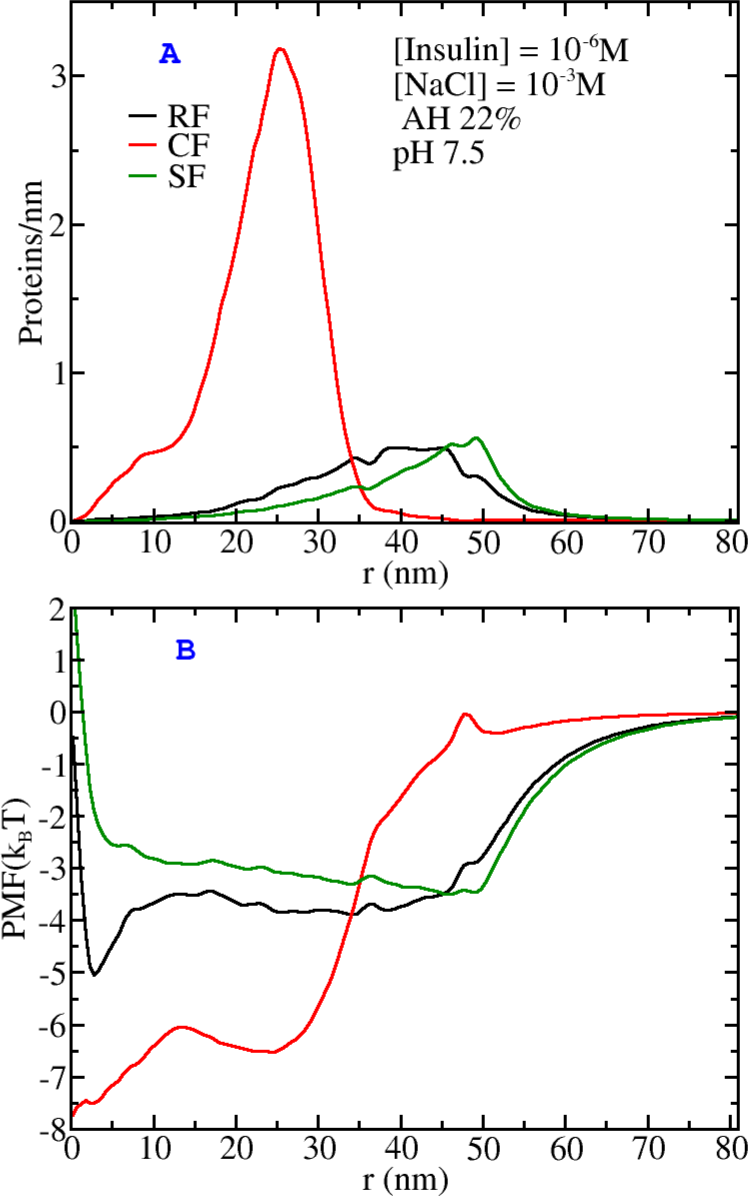
\includegraphics[width=0.45\textwidth]{Figures/graphs-gel2/insu-ads-pmf.png}
    \caption{A: Plot of the local distribution of insulin molecules, $\langle N(r)\rangle$, as a function of position for AH-VA nanogels having 22\% pH-sensitive segments in different network configurations.
    pH is 7.5, $10^{-6}$\,M insulin and  $10^{-3}$\,M NaCl.
    B: Potential of mean force,  ${PMF}(r)$, as a function of position for the same conditions as panel A.}
    \label{fig:adsorption-vs-r-insulin}
\end{figure}



Figura \ref{fig:adsorption-vs-r-insulin}A shows how adsorbed proteins are spatially distributed inside the different AH-based nanogels with \%22 degree of functionalization.
The pH of these results corresponds to the adsorption maximum of Figura \ref{fig:adsorption-vs-pH-insulin}A.
Insulin adsorption to the CF nanogel is not only significantly higher than the adsorption to the RF and SF nanogels, but it also occurs deeper inside the structure.
The most likely position of an insulin molecule occurs around $r=25$\,nm for the CF nanogel,
while this position moves to around $40-45$ and 50\,nm for the RF and SF structures respectively.




For MAA-based nanogels, Figura \ref{fig:adsorption-vs-r-cyto}A shows relatively minor differences between the distributions of cytochrome c inside RF and SF networks.
Such are differences slightly accentuated for insulin adsorption to the AH-VA nanogels, as seen in Figura \ref{fig:adsorption-vs-r-insulin}A.
Insulin distribution is displaced to the interior of the network in the randomly modified nanogel as compared to the surface functionalization, where proteins are more likely to occupy the very vicinity of polymer-solution interface.
Overall insulin distribution profiles are still relatively similar for these two structures.
These results show, once again, that network design (polymer synthesis) provides a tool to control the distribution of proteins inside the nanogel.






Panel B of figura \ref{fig:adsorption-vs-r-insulin} shows the potential of mean force acting on insulin molecules at the same conditions as panel A.
The attractive interaction on adsorbed insulin ranges from $-8$ to $-6 k_B T$ inside the CF structure and from $-5$ to $-4 k_B T$ inside RF nanogel.
Inside the SF nanogel the potential presents a minimum of $-4 k_B T$  at the surface and then increases monotonously as $r$ decreases inside the gel.







%%%%%%%%%%%%%%%%%%%%%%%%%%%%%%%%%%%%%%%%%%%%%%%%%%
\section{Conclusions}
%%%%%%%%%%%%%%%%%%%%%%%%%%%%%%%%%%%%%%%%%%%%%%%%%%


We have presented a study of protein adsorption to polymer nanogels having  different pH-responsive functionalizations.
We have derived and applied a thermodynamic theory that can be informed by a coarse-grained molecular model.

The 



